\documentclass[12pt,halfline,a4paper]{ouparticle}
\usepackage[utf8]{inputenc}
\usepackage[english]{babel}
\usepackage[
backend=biber,
style=alphabetic,
sorting=ynt
]{biblatex}
\usepackage[nottoc]{tocbibind}

\addbibresource{paper.bib}

\begin{document}

\title{Using a Two-Layer Neural Network and Physicochemical Properties to Classify Glass for Forensic Analysis}

\author{%
\name{Michael Arango}
\email{mikearango@gwu.edu}
	\and
\name{Mark Barna}
\email{mark.barna@gmail.com}
	\and
\name{Paul Brewster}
\email{pfbrewster@gmail.com}
}

%\abstract{abstract text goes here...}
\date{\today}
\maketitle
\pagebreak
\tableofcontents
\pagebreak

\section{Project Proposal}
\label{sec1}
In this study, we will use the physicochemical properties of glass to determine whether or not a given glass sample was taken from a window. This is a fundamental problem in forensic analysis as it is highly unlikely that glass fragments will be found on people unless they have been present at the time glass breaks. Glass analysis is of vital importance in forensic science as it allows us to test if the glass fragment found on a person is the same as the glass at a crime scene. Since glass is made up of several raw materials and certain elements impart specific properties, we can find out a lot about the glass if we analyze the chemical composition.

The dataset we chose for analysis was made available for download from the UCI Machine Learning Repository and was created by the USA Forensic Science Service. There are 214 observations of 9 different features along with 214 targets that specify whether the glass sample came from a window or not. While we would like more data to train a neural network, we believe the dataset is large enough for our purposes. It is difficult to know before we train a neural network if we have enough data, but the amount of data required is directly related to the complexity of the underlying decision boundary we are trying to implement. We won't 
know how complex the decision boundary we are trying to approximate is until we train the network, but we feel confident using the dataset as many others have used the dataset and found robust results. Several other papers in the literature use much more complex methods than we will employ and have not found the size of the data to be an issue. 

We have chosen a two-layer perceptron network with tangent-sigmoid transfer functions in the hidden layer and \emph{softmax} transfer functions in the output layer. This is a fairly standard network for pattern recognition. Moreover, we will use the \emph{Scaled Conjugate Gradient (SGD)} algorithm to train the network as it is good for pattern recognition problems in which the output layer uses a non-linear transfer function. Since we do not expect the training error to converge to zero, we implement early stopping criteria to prevent overfitting. Lastly, we use \emph{cross-entropy} as our performance index since our targets take on discrete values and it is the optimal performance index for pattern recognition networks that use the \emph{softmax} transfer function in the output layer. 

Two different frameworks will be used to implement the neural network. First, we will use the Neural Network Toolbox, specifically the Neural Network Pattern Recognition Tool (\verb|nprtool|) train, validate, and test our network. We use this framework to start with a simple graphical user interface to quickly ensure our specified network architecture is appropriate and to get baseline performance statistics. Then, we will replicate the analysis in Python to gain practical experience building network architectures in a scripting language. Note that since the goal is practical experience, we will not be leveraging the power of the \emph{scikit-learn} package (\verb|sklearn|) for this exercise. 

Several reference materials will be consulted to obtain sufficient background knowledge of the subject at hand. First, we plan on doing a thorough review of the forensic chemistry and geology literature to understand the reasons for using physicochemical properties to classify glass. Then, papers on glass analysis will be examined to supplement background knowledge with experiential knowledge. 

Considering our problem is one of pattern recognition, a confusion matrix will be used to assess the accuracy of our model and the \emph{false postive} (Type I error) and \emph{false negative} (Type II error) rates. Further, the \emph{Receiver Operating Characteristic (ROC) curve} will be used to compare the true positive rate to the false positive rate. This will help us gain additional knowledge of the predictive power of our network. 

We plan to finish our research and submit it by Wednesday, June 28, 2017. 

\section{Introduction}
\label{sec2}
An overview of the project and an outline of the report (I like to write intro after I finish a project).

\subsection{Literature Review}
\label{sec2.1}
The dataset we will use for this analysis was initially employed in Evett and Spiehler's paper \emph{Rule Induction in Forensic Science} (1987) \cite{evett1987}. They recognized the usefulness to a forensic crime lab of classifying glass fragments based on refractive index and chemical composition. This would, for example, allow the lab to ascertain whether samples gathered on a suspect?s clothing came from a window, potentially indicating they had broken it, or from another source, like a broken bottle. 

In their experiment, Evett and Spiehler wished to see if the Bionic Evolutionary Algorithm Generating Logical Expressions (BEAGLE) machine learning algorithm could correctly classify the glass---first as either window or non-window, and then into a second level of sub-categories. Our project focuses on the former and leaves the latter as a future exercise. The BEAGLE algorithm Evett and Spiehler used to train the network uses a series of logical ``and'' statements to chain rules together based on the inputs. They offer up the following example of a rule: 
\[ 
\{(\mathrm{Fe} \leq \mathrm{Na}) \text{ and } [\mathrm{K} > (\mathrm{Fe} \cdot 650)]\}, 
\]
where $\mathrm{Fe}$, $\mathrm{Na}$, and $\mathrm{K}$ are the percent composition of iron, sodium, and potassium, respectively, of each glass sample. Evett and Spiehler found that the BEAGLE algorithm outperformed the $k$-Nearest Neighbors algorithm (with $ k = 3$) and Linear Discriminant Analysis (LDA)---the models they used for baseline performance measures. 

The Department of Justice regularly issues research grants for the elemental analysis of glass. In 2012, they issued one such grant to researchers at Florida International University (FIU) to work with the Miami-Dade County Police Department \cite{almirall2012}. The researchers note that analysis of small quantities of materials has become an important yet underutilized type of evidence at many crime scenes including hit-and-run accidents and other violent crimes. The ability to classify different types of glass could be of vital importance in the case of a hit-and-run. Further, the group of researchers attempted to compare the discrimination power between the methods used in most forensic laboratories for glass analysis. Their aim was to create a more ``standard'' method that can be used by the operational forensic laboratory and a ``match criteria'' for use in routine casework situations.

Maureen Bottrell, a geologist and forensic scientist at the FBI Laboratory released a report in 2009 documenting the background information that ought to be used when comparing glass samples with data \cite{bottrell2009}. She notes that the vast majority of raw materials used to make glass are derived geologically and that North American glass makers use more than 20 million tons of raw materials annually. All of these materials contain several impurities that result in perceived differences in glass products. 

Bottrell writes that physical properties such as color, curvature, fluorescence, thickness, and surface features should first be used to determine if the material fragments are glass. Once we know a sample is glass, Bottrell recommends using optical properties, particle immersion, density, and elemental analysis to differentiate between types of glass. In this study, we focus on optical properties, specifically the refractive index, and elemental analysis to classify whether glass samples came from a window or not.\footnote{See section \ref{sec3.1} for more on the refractive index.}

Since glass is made up of several raw materials and certain elements impart specific properties, we can find out a lot about the glass if we analyze the chemical composition. Glass made on the same manufacturing line over a period of time can often have highly variable properties as mixtures of raw materials can have drastically different chemical compositions. 

\section{Description of the Dataset}
\label{sec3}
The dataset was made available for download from the UCI Machine Learning Repository and was created by the USA Forensic Science Service \cite{murphy1994}. The purpose of this dataset is to use physicochemical properties to classify whether a certain glass fragment comes from a window or not. 

\subsection{Inputs}
\label{sec3.1}
The matrix of inputs contains 214 observations of 9 variables and there is no missing data. Of these variables, eight of the nine measure the percent weight that a given elemental oxide makes up of the total glass sample weight. All the eight elements except silicon are classified as metals on the periodic table of elements. Sodium and potassium are alkali metals whereas magnesium, calcium, and barium alkaline earth metals. Aluminum and iron are classified as poor metals and transition metals, respectively. The last variable in the input matrix represents the refractive index which measures the speed of light in a transparent medium and is known as Snell's law. It can be represented formulaically as the ratio of the velocity of light in a vacuum to the velocity of light in the glass itself: $n = \frac{c}{v}$. A more thorough description of target variables is as follows: 
\begin{description}
\item \textbf{Refractive Index:}
measures the ratio of the velocity of light in a vacuum to the velocity of light in the glass itself
\item \textbf{Sodium:}
represents the percent weight in sodium oxide ($\mathrm{Na_{2}O}$)
\item \textbf{Magnesium:}
represents the percent weight in magnesium oxide ($\mathrm{MgO}$)
\item \textbf{Aluminum:}
represents the percent weight in aluminum oxide ($\mathrm{Na_{2}O}$)
\item \textbf{Silicon:}
represents the percent weight in silicon oxide ($\mathrm{Al_{2}O_{3}}$)
\item \textbf{Potassium:}
represents the percent weight in potassium oxide ($\mathrm{K_{2}O}$)
\item \textbf{Calcium:}
represents the percent weight in calcium oxide ($\mathrm{Ca_{2}O}$)
\item \textbf{Barium:}
represents the percent weight in barium oxide ($\mathrm{Ba_{2}O}$)
\item \textbf{Iron:}
represents the percent weight in iron oxide ($\mathrm{Fe_{2}O_{3}}$)
\end{description}

\subsection{Targets}
\label{sec3.2}
The matrix of targets has 214 observations, one for each observation in the training set, where a given target is denoted by $\begin{bmatrix} 1 \\ 0 \end{bmatrix}$ if the glass sample comes from a window and $\begin{bmatrix} 0 \\ 1 \end{bmatrix}$ otherwise. Note that the targets are two-dimensional instead of the more common one-dimensional binary encoding. This two-dimensional encoding allows us to have only one neuron firing at a time and tends to result in marginally better performance. 

\section{Description of the Network Architecture and Training Algorithm}
\label{sec4}
Once the data is preprocessed, the next step is to decide on or create a network architecture. The basic network architecture is determined by the problem we wish to solve. Once the basic network architecture is determined, we decide how many layers, how many neurons in each layer, how many outputs the network should have, and what kind of performance index function we should use for training \cite{hagan2014}. 

\subsection{Network Architecture}
\label{sec4.1}
The standard neural network architecture for pattern recognition problems is the multi-layer perceptron with tangent-sigmoid transfer functions in the hidden layers and \emph{softmax} transfer functions in the output layer. For most problems, including a fairly simple one like ours, one hidden layer usually suffices. Thus, we will implement a two-layer perceptron. If the results of the network are unsatisfactory after training and testing with one hidden layer, we will retrain with an additional hidden layer, but we do not anticipate having to do this. The \emph{tansig} transfer function is usually preferred to the \emph{tansig} transfer function in the hidden layers since it produces outputs (which are inputs to the next layer) that are centered near zero, whereas the \emph{tansig} transfer function always produces positive outputs. 

We also need to select the number of neurons in each layer. The number of neurons we use in the output layer should be the same as the size of the target vector. In our case, this means we should use two neurons in the output layer. On the other hand, the number of neurons we use in the hidden layer is directly proportional to the the complexity of the decision boundary being implemented. Since we do not know the complexity of the decision boundary needed to classify these glass samples before training, we begin with ten neurons, which may be more than we need, and leverage early stopping techniques to prevent overfitting \cite{hagan2014}. 

Now that we have chosen a network architecture, we can calculate the network output. The output from the hidden layer (the input to the output layer) can be calculated as 
\[
\mathbf{a^{1}} = \textbf{tansig}(\mathbf{W^{1}}\mathbf{p} + \mathbf{b^{1}}), 
\] 
while the output from the output layer is 
\[ 
\mathbf{a^{2}} = \textbf{softmax}(\mathbf{W^{2}}\mathbf{a^{1}} + \mathbf{b^{2}}). 
\]
The network architecture can be seen in \textbf{Figure 1} below. 
\begin{figure}[H]
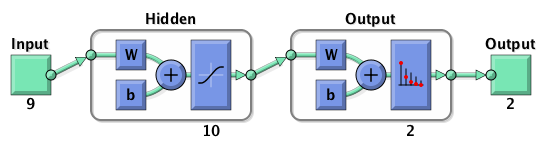
\includegraphics[width = 6in]{figs/network.png}
\caption{Two-Layer Perceptron Used to Classify Glass Samples}
\end{figure}

\subsubsection{History of the Perceptron}
\label{sec4.1.1}
Before discussing the training algorithm, we offer up a brief history of the perceptron. Much of the modern interpretation of neural networks is credited in large part to Warren McCulloch and Walter Pitts who showed that networks of artificial neurons could calculate any function. We still use the fundamental feature of their model in which a weighted sum of inputs is compared to a threshold to determine the output of a neuron \cite{hagan2014}.

One of the first applications of neural networks came in the 1950's when Frank Rosenblatt developed the perceptron network and the corresponding learning rule to solve pattern recognition problems. While his developments were monumental at the time, several researchers showed that a single-layer perceptron and the learning rule could not solve certain problems. Specifically, the error will never converge to zero when using the perceptron learning rule if the input vectors are \emph{linearly inseparable}. It wasn't until the 1980's that multi-layer perceptron networks and more complex learning rules were proposed that could solve these problems. 

%Widrow and Hoff's learning rule suffered from the same disadvantage. When we have more complicated decision boundaries we are trying to implement and have multiple layers, a more robust learning rule ought to be used. Since then, multilayer perceptrons trained by the backpropagation algorithm have become the most popular neural network. \cite{hagan2014}. 

\subsection{Training Algorithm}
\label{sec4.2}
We chose to use the Scaled Conjugate Gradient (SCG) algorithm to train our network as it is very efficient for pattern recognition problems. For multi-layer networks, the Levenberg-Marquardt algorithm is often used, but it does not work well for pattern recognition as the transfer function in the output layer is operating outside the linear region. The scaled conjugate gradient algorithm is a special type of backpropagation. In backpropagation, we adjust the weights in the direction of steepest descent... 


\section{Experimental Setup}
\label{sec5}

\subsection{Data Preprocessing}
\label{sec5.1}

\subsection{Implementation of the Network}
\label{sec5.2}

\subsection{Performance Index}
\label{sec5.3}

\section{Results}
\label{sec6}

\section{Conclusion}
\label{sec7}


\pagebreak

\printbibliography[heading=bibintoc, title={References}]

\pagebreak
\appendix

\section{Perceptron}
\section{Backprop}
\section{Subroutine X}

\end{document}
